\documentclass[tikz]{standalone}
\standaloneconfig{border=0.3cm}
\usepackage{tikz}
\usetikzlibrary{shapes, automata, arrows, positioning, fit, backgrounds, shapes.geometric, matrix}
\tikzstyle{block} = [rectangle, draw,
    text width=9em, text centered, rounded corners, minimum height=3.5em]
\tikzstyle{bordertext} = [text centered, rotate=270]
\tikzstyle{line} = [draw, -latex']

\begin{document}

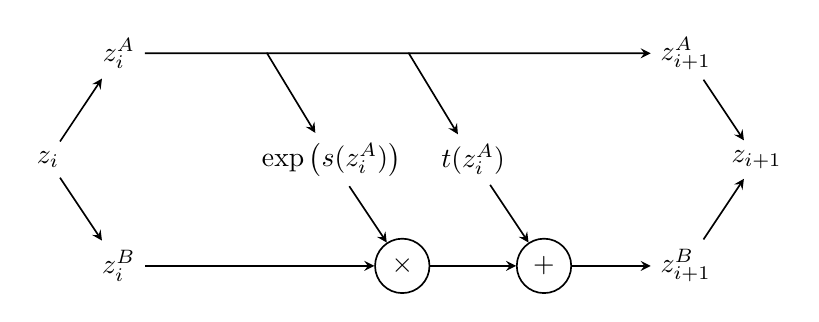
\begin{tikzpicture}[->,scale=1.8,
          > = stealth, % arrow head style
          shorten > = 0, % don't touch arrow head to node
          auto,
          node distance = 3cm, % distance between nodes
          semithick % line style
      ]

      \tikzstyle{every state}=[
          draw = black,
          semithick,
          fill = white,
          minimum size = 4mm
      ]
  % Draw the vertices.
  \node (a) at (0.5, 0.75) {$z_i$};

  \node (c) at (1, 1.5) {$z_i^A$};
  \node (d) at (2, 1.575) {};
  \node (e) at (3, 1.575) {};
  \node (f) at (5, 1.5) {$z_{i+1}^A$};

  \node (b) at (1, 0) {$z_i^B$};
  \node[state] (g) at (3, 0) {$\times$};
  \node[state] (h) at (4, 0) {$+$};
  \node (i) at (5, 0) {$z_{i+1}^B$};

  \node (j) at (5.5, 0.75) {$z_{i+1}$};

  \node (k) at (2.5, 0.75) {$\exp \left(s(z_i^A)\right)$};
  \node (l) at (3.5, 0.75) {$t(z_i^A)$};

  % Connect vertices with edges and draw weights
  \path (a) edge node {} (b);
  \path (a) edge node {} (c);
  \path (b) edge node {} (g);
  \path (g) edge node {} (h);
  \path (h) edge node {} (i);
  \path (c) edge node {} (f);
  \path (i) edge node {} (j);
  \path (f) edge node {} (j);

  \path (d) edge node {} (k);
  \path (k) edge node {} (g);

  \path (e) edge node {} (l);
  \path (l) edge node {} (h);
\end{tikzpicture}

\end{document}
